
\section{CaraNet: Context Axial Reverse Attention Network for Segmentation of Small Medical Objects}

\subsection*{Ссылка} \url{https://arxiv.org/abs/2108.07368}
\subsection*{Введение}
 На данный момент разработано достаточное количество архитектур 
 сверточных сетей для решения задачи сегментации медицинских, которые 
 показывают хорошие результаты. Однако, только малая часть 
 исследований учитывает размер интересующих объектов на изображении
 и поэтому многие модели показывают плохой результат при сегментации
 объектов малого размера, что сильно влияет при диагностике заболевания.
 В данной работе предлагается нейросетевая модель Context Axial
 Reserve Attention Network (CaraNet), которая способна улучшить 
 результаты сегментации малых объектов по сравнению с уже существующими
 моделями.
\subsection*{Основная идея}
В архитектуре CaraNet используется параллельный частичный декодер 
(parallel partial decoder) для генерации высокоуровневой семантической
карты и набор операций (Context and Axial Reverse Attention) для 
идентификации глобальных и локальных признаков. 
\\Модули CaraNet:
\begin{itemize}
    \item \textit{Parallel partial decoder.} Эксперименты показали,
    что низкоуровненвые признаки вычислительно более сложны и вносят 
    меньший вклад в улучшение результатов сегментации. Поэтому, авторы 
    используют параллельный частичный декодер \(p_d(\cdot)\) для извлечения 
    высокоуровневых признаков \(PD=p_d(f_3,f_4,f_5)\) и получения глобальной карты 
    \(S_g\) из частичного декодера.
    \item \textit{Context module.} Чтобы получить контекстную информацию из высокоуровневых
    признаков, применяется модуль CFP (Channel-wise Feature Pyramid) cо степенью растяжения 
    (dilation rate) \(d=8\). После контекстного модуля можно получить многомасштабные 
    высокоуровневые признаки \(\{f_{3}^{'}, f_{4}^{'}, f_{5}^{'}\}\).
    \item \textit{Axial reverse attention.} Данный модуль состоит из двух частей:
    маршрут по оси (axial attention route) и обратный маршрут (reverse attention route). Глобальная 
    карта \(S_g\) может поймать только приблизительное расположение тканей без структурных деталей, 
    поэтому структурированный регион тканей постепенно добывается стиранием переднего плана 
    объекта с помощью операции reverse attention: \(R_{i}=1-Sigmoid(S_{i})\). По другому 
    маршруту применяется axial attention. Здесь сеть может извлечь глобальные зависимости и 
    локальное представление совершая вычисления по горизонтальной и вертикальной оси. 
\end{itemize}
\begin{minipage}{1.0\linewidth}
    \begin{center}
        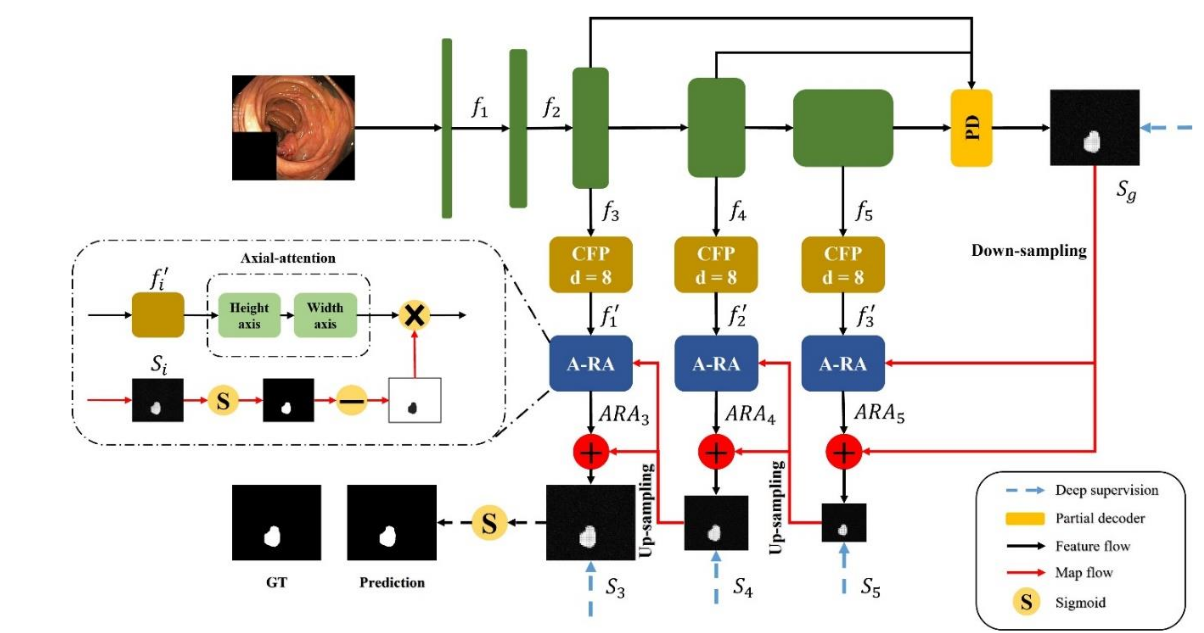
\includegraphics[scale=0.35]{ann8_arch.png} \\
        \caption{\scriptsize{Архитектура CaraNet, состоящая из трех контекстных модулей (CFP) и 
        модулей axial reverse attention (A-RA). 'S' - сигмоида.}}
    \end{center}
    
\end{minipage}
\subsection*{Данные}
\begin{itemize}
    \item BraTS 2018 - опухоли ГМ
    \item Kvasir-SEG, CVC-ColonDB, CVC-ClinicDB, CVC-
    300 and ETIS-LaribPolypDB - полипы
\end{itemize}
 
\subsection*{Результаты}
По сегментации полипов на основе пяти датасетов, предложенная модель CaraNet не только 
превосходит сравниваемые модели по общей производительности, но и на примерах с полипами 
малых размеров. \\
\\
\begin{minipage}{1.0\linewidth}
    \begin{center}
        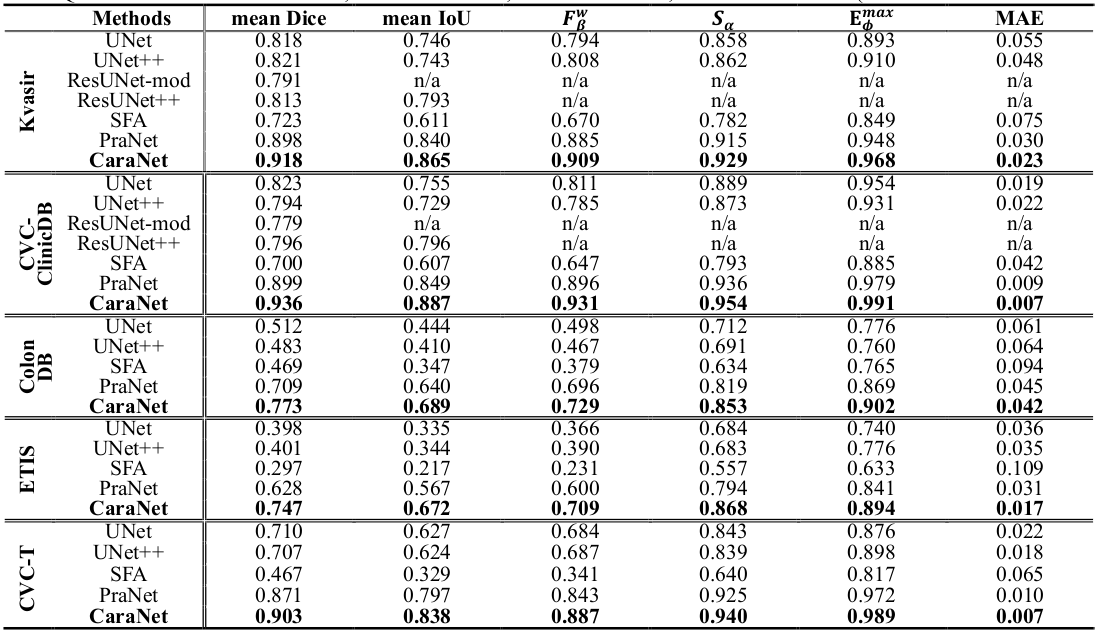
\includegraphics[scale=0.4]{ann8_res1.png}
        \caption{\scriptsize{Количественные результаты на Kvasir, CVC-ClinicDB, CVC-ColonDB, ETIS и CVC-T}}
    \end{center}
\end{minipage}

Для дальнейшей оценки эффективности сегментации малых объектов с помощью CaraNet был 
проведен еще один эксперимент, уже с участием опухолей ГМ из датасета BraTS 2018. CaraNet 
была сравнена с PraNet и показала лучший результат особенно в случаях с очень малыми объектами. \\
\\
\begin{minipage}{1.0\linewidth}
    \begin{center}
        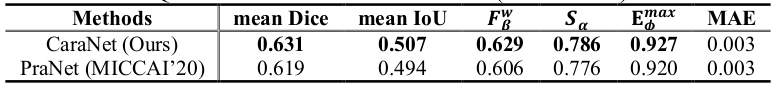
\includegraphics[scale=0.5]{ann8_res2.png} \\
        \caption{\scriptsize{Количественные результаты на датасете BraTS 2018}}
    \end{center}
    
\end{minipage}



\subsection*{Заключение}
Была предложена новая нейросетевая модель CaraNet, состоящая из комбинации моделей 
Axial Reverse Attention и Channel-wise Feature Pyramid, которая показала 
лучшие результаты сегментации малых объектов на медицинских изображениях по сравнению с уже существующими моделями 
UNet, UNet++, ResUNet-mod, ResUNet++, SFA, PraNet, что может внести большой вклад 
при постановке диагноза и выборе дальнейшей тактики лечения.